\section{Test generation}

Given an operation ${\cal O}$ and a rule part $r$ in that operation, the goal 
of our technique is to generate a test that covers the rule part $r$. In our setting,
a test includes a sequence of operations along with necessary data passed
as inputs to those operations. This sequence of operations produce all input entities
of ${\cal O}$ and also desired object states for all those entities that help cover
$r$. Identifying such desired sequence of operations
that covers $r$ is challenging due to a large search space of possible sequences.
For example, in the subject \subject{Cebu-pacific} airlines used in our evaluation,
there are eight operations that accept an entity called \subject{Ticket}
as input and modify that entity. Therefore,
any sequence composed using one or more of these operations is a valid sequence, however, different 
sequences and also different orderings of each sequence
produce different object states. To address this challenge, our 
technique efficiently explores the search space by incrementally composing
sequences.

In particular, our technique first enumerates
sequences of operations (along with selected rule parts in those operations) 
that create all entities required for invoking
the operation ${\cal O}$. Next, for each sequence, our technique checks whether
the sequence is satisfiable---i.e., whether the sequence generates desired
object states (for all input entities of ${\cal O}$) that help cover the
precondition of the rule part $r$. If the sequence is satisfiable, our technique
infers values for all variables of primitive and enumerated types passed as inputs to those operations
and generates a test. Otherwise, our technique identifies the entity $e$ 
and its attribute $attr$ that needs to be modified
to achieve the desired object state. Next, our technique identifies candidate
operations that modify $attr$ of the entity $e$, composes
new sequences using those candidate operations, and checks whether those
new sequences are satisfiable. Our technique repeats this
process until it identifies a satisfiable sequence or reaches user defined threshold
expressed in terms of the maximum number of sequences to be explored.

We next present the terminology and then explain the core algorithm of our technique.

\subsection{Terminology}

\subsubsection{Graphs}
We use two types of graph notations in our algorithm.

\textit{Dependency Graph.} A dependency graph is a directed graph that
captures interactions of operations with entities in the application.
Our graph includes three types of edges: {\tt create}, {\tt read}, and {\tt modify}.
A {\tt create} edge from an operation to an entity indicates that the operation
creates that entity. Similarly, {\tt read} and {\tt modify} edges indicate that
the operation reads or modifies the corresponding entity, respectively.
This graph is used while composing sequences to ensure that the dependencies among operations are satisfied.
Figure~\ref{fig:sample-app} shows the dependency graph for our example application.

\textit{Operation Flow Graph.} To identify combinations of rule parts (within an operation)
that help create different object states of entities, we model each operation as a control
flow graph. Since preconditions of all rule parts in
a rule are disjoint (see Sec~\ref{sec:model}, Property~1), control flow through a rule can cover
exactly one rule part. Our graph reflects this by
representing each rule as a choice among its rule parts. We create a flow graph for the entire
operation by sequencing individual components of each rule. 
Since there is no data dependence between rules in an operation (see Sec~\ref{sec:model}, Property~4),
all orderings are equivalent. Figure~\ref{fig:cfg} shows flow graph for 
the \subject{GenerateInvoice} operation with two rules, where $R_4$
and $R_5$ include three and two rule parts, respectively.

\subsubsection{Operation Sequences}
We next define two types of operation sequences that are used to explain
our algorithm.

\textit{Abstract Sequence.} An abstract sequence is a sequence of operations describing
flow of objects among those operations. Within the sequence, all variables
of type \subject{Object} (i.e., non-primitive) should be defined and other variables of enumerated and primitive types are not
defined. An example abstract sequence for \subject{GenerateInvoice} is shown below.

\vspace*{-5pt}
{\small
\begin{alltt}
  State st; BalanceType bt; int price;
  CreateCustomer(st, bt, out Customer cust);
  CreateOrder(cust, out Order ord);	
  CreateItem(price, out Item item);
  AddItemToOrder(ord, item, out Order ord1);
  GenerateInvoice(ord1, out Invoice inv);  
\end{alltt}
}
\vspace*{-5pt}

In our notation for an abstract sequence, variables that are created or modified by each operation
are represented using the \subject{out} keyword, whereas other variables 
are inputs to that operation. As shown, all variables of \subject{Object} types
are initialized within the sequence. 

\textit{Concrete Sequence.} A concrete sequence is similar to an abstract sequence, but
includes selected set of rule parts in each operation. Our technique builds a boolean formula
from concrete sequences using preconditions and postconditions of all rule parts, and uses
constraint solver to check whether the formula is satisfiable. An example concrete
sequence for the preceding abstract sequence is shown below. The rule parts selected in each 
operation are shown next to that operation.

\vspace*{-5pt}
{\small
\begin{alltt}
  State st; BalanceType bt; int price;
  CreateCustomer(st, bt, out Customer cust) [\(r\sb{1.1}\)];
  CreateOrder(cust, out Order ord) [\(r\sb{3.1}\)];	
  CreateItem(price, out Item item) [\(r\sb{2.1}\)];
  AddItemToOrder(ord, item, out Order ord1) [\(r\sb{7.1}\)];
  GenerateInvoice(ord1, out Invoice inv) [\(r\sb{4.1}\)];  
\end{alltt}
}
\vspace*{-5pt}

\begin{figure}
\centering
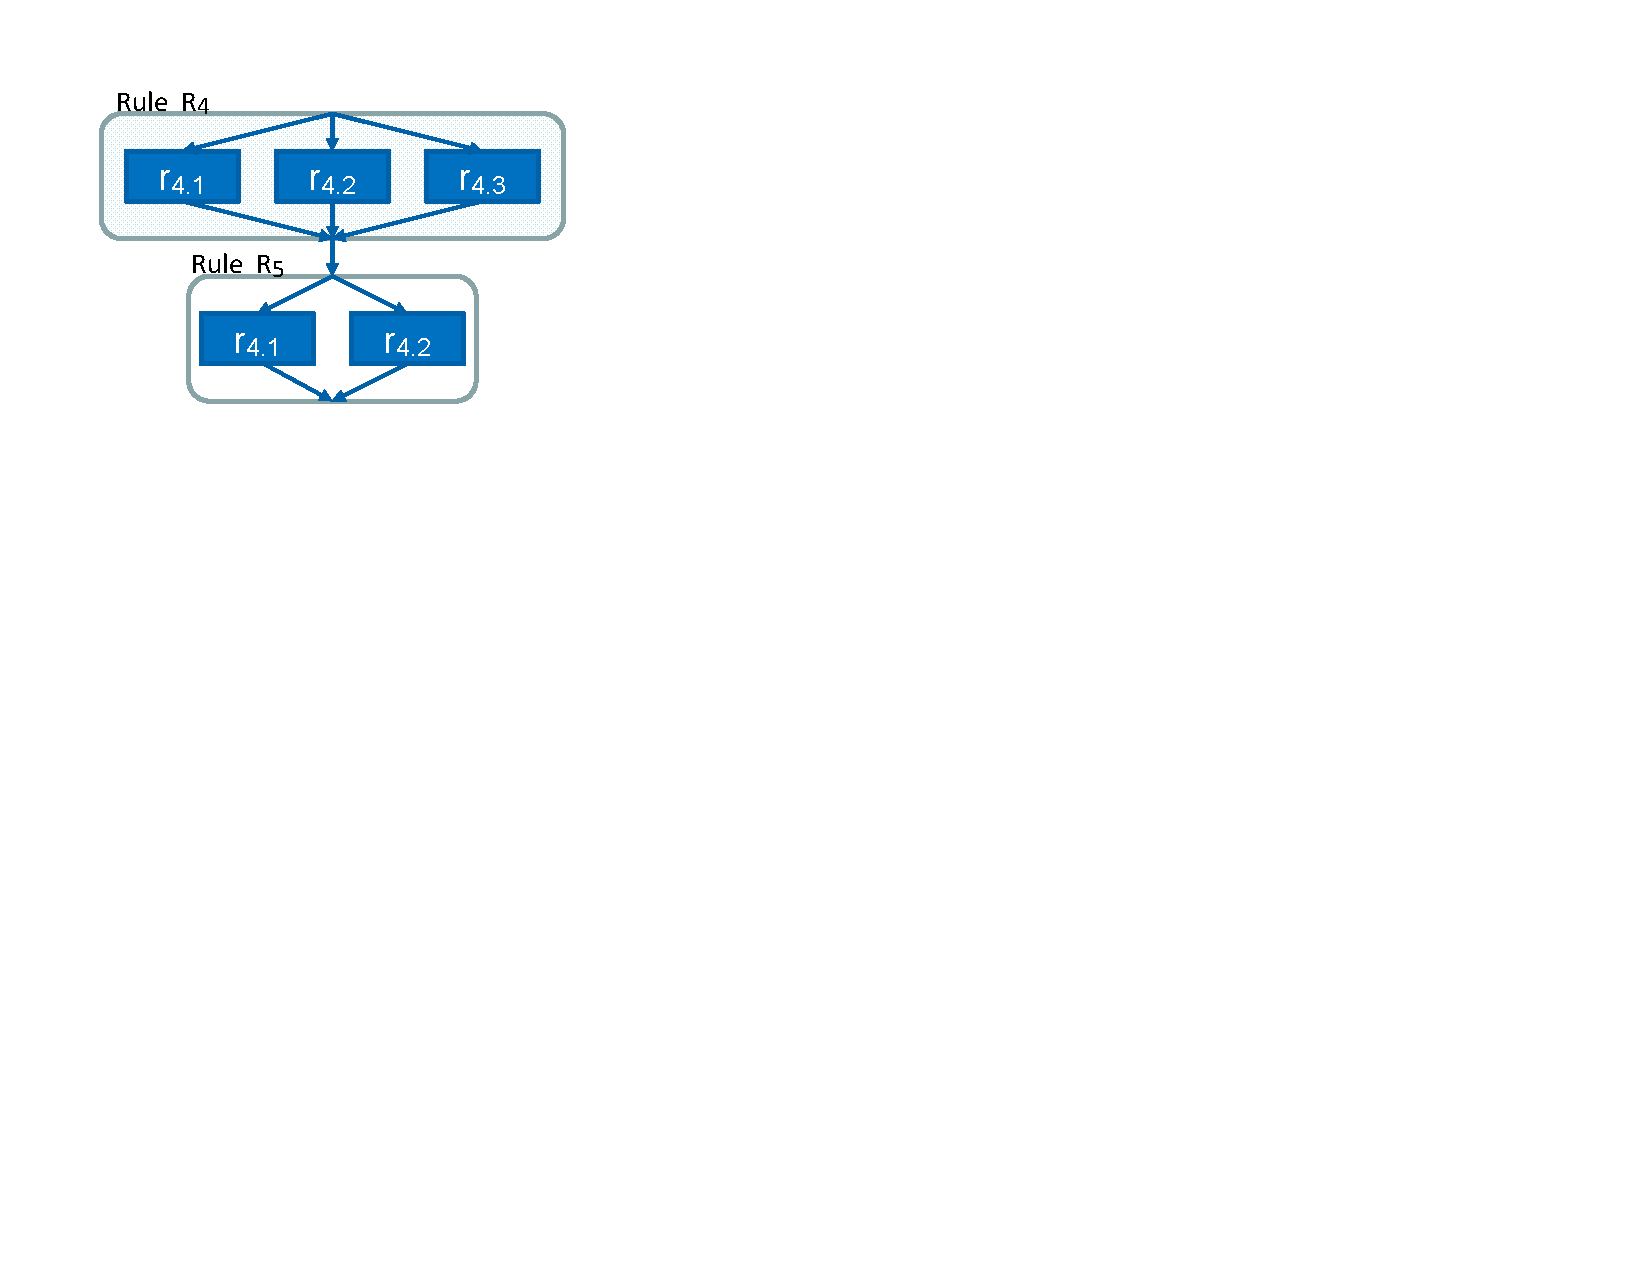
\includegraphics[trim=48 390 520 38,clip,width=2in]{figs/cfg-example.pdf}
\caption{Operation flow graph for the \subject{GenerateInvoice} operation.}
\label{fig:cfg}
\end{figure}

\begin{algorithm}[t]
\footnotesize
\SetAlgoVlined
\KwIn{Operation ${\cal O}$, Rule part $r$}
\KwOut{ConcreteSequence $seq$ or $null$}
\BlankLine

\nl Initialize a Queue $queue$ for storing concrete sequences\;
\nl Generate all constructor sequences $cseqList$ for ${\cal O}$\;
\nl \ForEach {constructor sequence $cseq \in cseqList$}
{
		\nl Generate all concrete sequences $conSeqList$ for $cseq$\;
		\nl Add all sequences in $conSeqList$ to $queue$\;
} 

\nl \While { queue not empty }
{
		\nl Remove the first concrete sequence $conSeq$ from $queue$\;
		\nl Check whether $conSeq$ is satisfiable\;
		\nl \If {satisfiable}
		{
				\Return $conSeq$ \;
		}
		
		\nl Extract unsatisfiable core $unSatCore$ of $conSeq$\;
		
		/*Ensures that selected operation helps to make progress*/
		\nl \If {$unSatCore$ is already seen}
		{
				Continue\;
		}
		
		\nl Identify operations $opSet$ that help cover $unSatCore$\;		
		\nl \ForEach {Operation $candOp$ $\in$ $opSet$}
		{
			\nl Insert $candOp$ in $conSeq$ to generate a list of new concrete sequences $seqList$\;
			\nl Add all sequences in $seqList$ to $queue$\;			
		}
}

\Return $null$\;
		
\caption{\label{alg:guidedsearch} Algorithm for
  identifying a concrete sequence that cover a given rule part.}
\end{algorithm}



\subsection{Algorithm}
\label{sec:technique}

Algorithm~\ref{alg:guidedsearch} shows the core algorithm of our technique. For illustration
purposes, we consider operation ${\cal O}$ as \subject{GenerateInvoice} and 
rule part $r$ as $r_{4.2}$. For brevity,
we omit details such as exiting the main loop (lines 6-15) when user-defined
threshold of maximum number of sequences to be explored is reached.

\textit{Generate Constructor Sequences (Lines 2--5).} Given an operation ${\cal O}$, our algorithm
first generates constructor sequences that produce all input entities of ${\cal O}$
using the dependency graph of the application.
Here, a constructor sequence is the same as an abstract sequence, however, includes only those
operations that create entities and does not include operations that modify
entities. In particular, our algorithm first identifies all input entities 
$E = \{e_1, e_2, \ldots, e_m\}$ of ${\cal O}$ through \textit{read}
edges in the graph. For each entity $e_i$, it identifies set of operations 
$OP_i = \{{\cal O}^i_1, {\cal O}^i_2, \ldots, {\cal O}^i_n\}$
that create $e_i$ through \textit{create} edges in the graph. Note that our model
allows multiple operations to create an entity. Next, our algorithm produces
combinations of all operations across each set corresponding to $e_i$ 
to generate constructor sequences. If there are $m$ input entities
and $n$ operations that create each entity, our algorithm generates $m * n$
constructor sequences. Note that the order of operations 
among these sequences does not matter, since they create different entities.
Next, our algorithm checks whether any operations in each $OP_i$
further requires additional entities, and repeats this process until no 
new input entities are required in all constructor sequences. 
For our illustrative example, the constructor sequence for 
\subject{GenerateInvoice} is shown below.

\vspace*{-5pt}
{\small
\begin{alltt}
  State st; BalanceType bt;
  CreateCustomer(st, bt, out Customer cust);  
  CreateOrder(cust, out Order ord);
  GenerateInvoice(ord, out Invoice inv);  
\end{alltt}
}
\vspace*{-5pt}

Next, from each constructor sequence,
our algorithm generates concrete sequences by computing all possible combinations of
rule parts among operations in the sequences. To achieve this, our algorithm
joins operation flow graphs corresponding to each individual operation in the sequence and then
enumerates all paths in the final flow graph. These concrete sequences generate different
object states for input entities of the operation ${\cal O}$. In our experience,
the number of constructor (and the concrete sequences generated from those
constructor sequences) sequences is low, since the number of operations 
that create entities is often quite low. For our current example,
there is only one concrete sequence, since each operation in the
preceding constructor sequence includes only one rule part.

\vspace*{-5pt}
{\small
\begin{alltt}
  State st; BalanceType bt;
  CreateCustomer(st, bt, out Customer cust) [\(RP\sb{1.1}\)];
  CreateOrder(cust, out Order ord) [\(RP\sb{3.1}\)];	
  GenerateInvoice(ord, out Invoice inv) [\(RP\sb{4.2}\)];  
\end{alltt}
}
\vspace*{-5pt}

\textit{Check Satisfiability (Line 8).} Next, our algorithm checks whether 
each concrete sequence in the queue is satisfiable. A concrete sequence 
is considered as satisfiable if it generates desired
object states for all input entities of ${\cal O}$ that help cover the precondition of the rule
part $r$. To achieve this, our algorithm constructs a formula composed
of constraints in preconditions and postconditions in each rule part of the sequence
and then leverages a constraint solver to check whether the composed
formula is satisfied or not.

For illustration purposes, consider the sequence of operations and their selected
rule parts as $({\cal O}_1 [r_{1.1}], {\cal O}_2 [r_{2.1}], \ldots, {\cal O}_n [r_{n.1}], {\cal O} [r])$.
Our algorithm starts with the precondition of $r$ (referred to as $target$) in the operation ${\cal O}$. 
It next generates binding constraints that substitute the entities
consumed by ${\cal O}$ by the entities created or
modified by the predecessor operation ${\cal O}_n$. These binding constraints bind 
the identifiers in the postcondition of $r_{n.1}$ to the identifiers of same type
in the precondition of $r$. As the solver has no
notion of objects, binding must also ensure that referenced object attributes
are appropriately bound.

Binding constraints are generated as follows. Let $v$ be an
identifier of type $\tau$ occurring in either the creates or modifies
clause of ${\cal O}_n$ and let $w$ be an identifier of the same type
occurring in the input clause of ${\cal O}$. If $\tau$ is an enumerated or primitive type,
the only binding needed is $w = v$. If $\tau$ is an object type, then
we must bind all attributes as well, yielding the following constraint.

$b_n$: $w = v \wedge w.f_1 = v.f_1 \wedge \ldots \wedge w.f_n = v.f_n$ 

Here, $f_1, \ldots , f_n$ are attributes of $\tau$. If any of the
fields are of object types themselves, this process is applied
recursively on each such attribute to generate the final binding
constraint. Using binding constraints, our algorithm generates the formula as $p_{n.1} \wedge q_{n.1}
\wedge b_n \wedge p$, where $p_{n.1}$ and $q_{n.1}$ are pre- and postconditions
of rule part $r_{n.1}$. Our algorithm leverages a 
constraint solver to check whether the composed formula is satisfiable.
If yes, it proceeds further by considering
this formula as $target$ and ${\cal O}_{n-1}$ as the predecessor operation.
Once it processes all operations in the sequence and if the formula is satisfiable,
it extracts values for variables of primitive and enumerated types
from the solver result to construct the test. 

For our running example, the solver returns that the composed formula
as unsatisfiable. The reason is that $r_{3.1}$ of \subject{CreateOrder} 
assigns zero to \subject{total} of the \subject{Order} entity, whereas the
precondition in rule part $r_{4.2}$ of \subject{GenerateInvoice} requires the value of \subject{total} 
as greater than zero.

\textit{Extract Unsatisfiable Core (Line 10).} If the composed formula is unsatisfiable,
our algorithm extracts the unsatisfiable core of the formula. An unsatisfiable core 
is a subset of the entire formula, which preserves the unsatisfiability but is simplified
compared to the original formula. This core helps identify additional operations that modify attributes of entities
to produce desired object states. In our current example, our algorithm extracts 
unsatisfiable core as \subject{ord.total = 0 $\wedge$ ord.total > 0}, composed of constraints
in rule parts $r_{3.1}$ and $r_{4.2}$. 

%If the unsatisfiable core is already seen for this sequence, our algorithm
%ignores the sequence. The reason is that the candidate operation that is suggested
%earlier did not help make any additional progress by resulting in the same unsatisfiable core.
%TODO: Refer to Tao's DSN paper for fitness functions.

\textit{Suggest Alternate Sequences (Lines 12--15).} Once the unsatisfiable core is extracted,
our algorithm identifies constraints, referred to as $c$, in the core that are contributed by the preceding operation
such as ${\cal O}_{n}$. The key intuition is to identify candidate operations
that satisfy the negation of $c$ so that the composed formula can be satisfiable.
To achieve this, our algorithm first extracts entities and their attributes involved
in $c$. Next, it identifies candidate operations that modify those entities.
Within each such candidate operation, our algorithm identifies rule parts 
that modify desired attributes and also whose
postconditions are compatible with the negation of $c$, i.e., $q \wedge \neg c$
is satisfiable.

%TODO: write about searching operations that modify parent entites as well.

Once a candidate operation (along with relevant rule parts) is identified, our algorithm
checks whether all input entities of the candidate operation are produced
in the sequence. If not, it identifies the additional operations that create the necessary
entities. Next, our algorithm composes new concrete sequences by inserting the candidate operation.
Note that there may be multiple sequences possible since the candidate operation can be inserted
at different places within the sequence. Our algorithm next adds all new sequences to the queue.

For our illustrative example, our algorithm identifies candidate operation as \subject{AddItemToOrder}
since this is the only operation that modifies \subject{Order} entity and its attribute \subject{total}.
Since this operation requires an additional entity \subject{Item} that does not exist
in the sequence, our algorithm adds the operation \subject{CreateItem} as well. After creating
the new concrete sequence, our algorithm checks satisifiability of the new sequence,
where it further detects the unsatisfiable core as \subject{cust.crLimit = 0 $\wedge$ cust.crLimit > 0}. 
Our algorithm repeats the loop 6--15, and identifies the final concrete sequence that help cover rule part $r_{4.2}$ as
follows:

\vspace*{-5pt}
{\small
\begin{alltt}
  State st; BalanceType bt; int price; int crLimit;
  CreateCustomer(st, bt, out Customer cust) [\(RP\sb{1.1}\)];
  AddCreditLimit(cust, crLimit, out Customer cust1) [\(RP\sb{6.1}\)];
  CreateOrder(cust, out Order ord) [\(RP\sb{3.1}\)];
  CreateItem(price, out Item item) [\(RP\sb{2.1}\)];
  AddItemToOrder(ord, item, out Order ord1) [\(RP\sb{7.1}\)];
  GenerateInvoice(ord1, out Invoice inv) [\(RP\sb{4.2}\)];  
\end{alltt}
}
\vspace*{-5pt}

